%%%%
%%%% Main Matter
%%%%

\addstarredpart{Part Zero}

\cleardoublepage
\chapter*{Table des matières}
\parttoc

%\addcontentsline{toc}{xpart}{}
%\addcontentsline{tdm}{section}{Tututututu}

\chapter[Introduction]{Introduction}
\section{Toto}
\section{titi}

\chapter[Présentation de mes travaux]{Presentation of my work}







%silly talks

\begin{figure}[!htb]
\begin{center}
\begin{turn}{270}
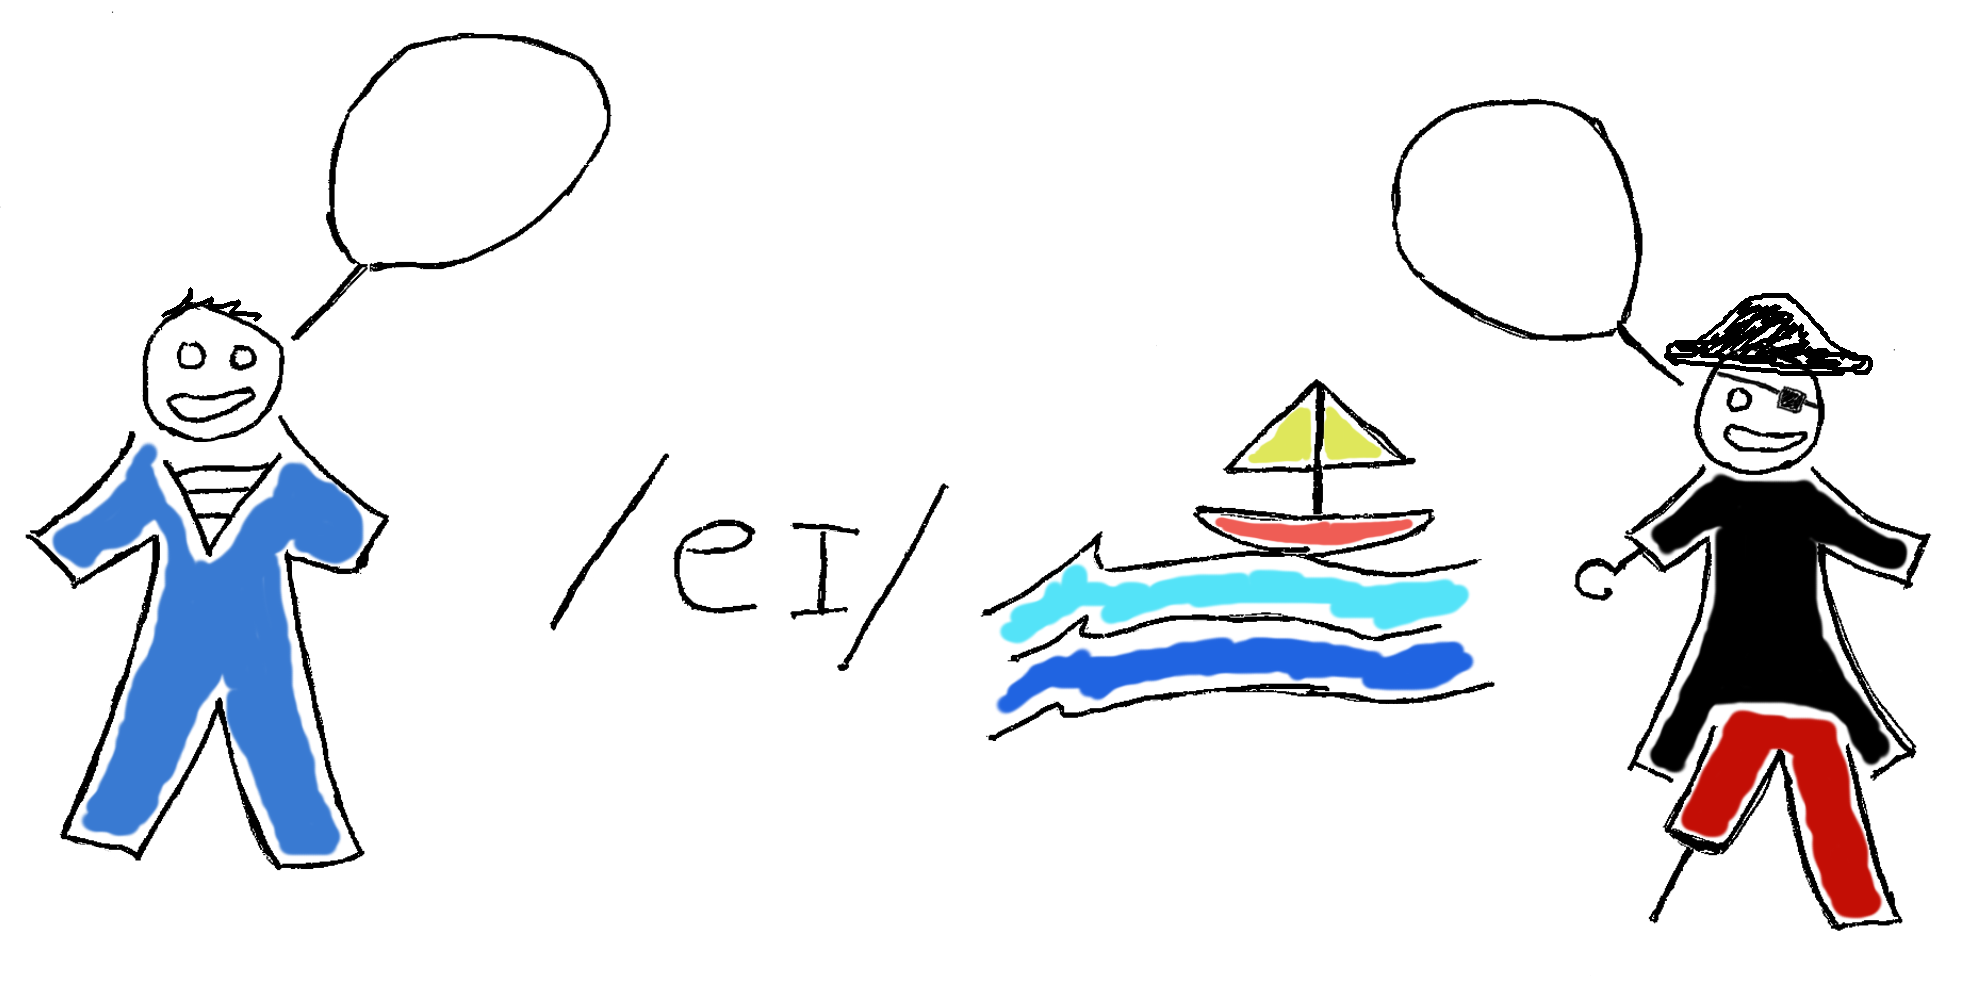
\includegraphics[scale=0.8]{iacr_coloured.png}
\end{turn}
\end{center}
\caption{A new flag for the IACR.\label{fig:iacr_flag}}
\end{figure}


\newcommand{\mybibtitle}[1]{\textsf{#1.}\hfil}
\newcommand{\mybibauth}[1]{#1.}
\newcommand{\mybibconf}[1]{\hspace*{\stretch{1}}\mbox{(#1)}}
\newcolumntype{z}{p{5em}}

\section[Mes publications]{My publications}

\subsection{Article de journal}

\noindent
\begin{tabularx}{\linewidth}{zX}
  \cite{asasajour} &
  \mybibtitle{Key-Recovery Attacks on ASASA}
  \mybibauth{B.~Minaud, P.~Derbez, P.-A.~Fouque, P.~Karpman}
  \mybibconf{Invité au J. Cryptology} \\
\end{tabularx}

\subsection{Articles de conférences}

\noindent
\begin{tabularx}{\linewidth}{zX}
  \cite{puppycipher} &
  \mybibtitle{Efficient and Provable White-Box Primitives}
  \mybibauth{P.-A.~Fouque, P.~Karpman, P.~Kirchner, B.~Minaud}
  \mybibconf{ASIACRYPT 2016} \\[2ex]
  \cite{DBLP:conf/eurocrypt/StevensKP16} &
  \mybibtitle{Freestart Collision for Full SHA-1}
  \mybibauth{M.~Stevens, P.~Karpman, T.~Peyrin}
  \mybibconf{EUROCRYPT 2016} \\[2ex]
  \cite{DBLP:conf/asiacrypt/MinaudDFK15} &
  \mybibtitle{Key-Recovery Attacks on ASASA}
  \mybibauth{B.~Minaud, P.~Derbez, P.-A.~Fouque, P.~Karpman}
  \mybibconf{ASIACRYPT 2015} \\[2ex]
  \cite{DBLP:conf/isw/Karpman15} &
  \mybibtitle{From Distinguishers to Key Recovery: Improved Related-Key Attacks on Even-Mansour}
  \mybibauth{P.~Karpman}
  \mybibconf{ISC 2015} \\[2ex]
  \cite{DBLP:conf/crypto/KarpmanPS15} &
  \mybibtitle{Practical Free-Start Collision Attacks on 76-step SHA-1}
  \mybibauth{P.~Karpman, T.~Peyrin, M.~Stevens}
  \mybibconf{CRYPTO 2015} \\[2ex]
  \cite{DBLP:conf/crypto/EspitauFK15} &
  \mybibtitle{Higher-Order Differential Meet-in-the-middle Preimage Attacks on SHA-1 and BLAKE}
  \mybibauth{T.~Espitau, P.-A.~Fouque, P.~Karpman}
  \mybibconf{CRYPTO 2015} \\[2ex]
  \cite{DBLP:conf/sacrypt/AugotFK14} &
  \mybibtitle{Diffusion Matrice from Algebraic-Geometry Codes with Efficient SIMD Implementation}
  \mybibauth{D.~Augot, P.-A.~Fouque, P.~Karpman}
  \mybibconf{SAC 2014} \\[2ex]
  \cite{DBLP:conf/ctrsa/0001KNWW14} &
  \mybibtitle{Analysis of BLAKE2}
  \mybibauth{J.~Guo, P.~Karpman, I. Nikolić, L. Wang, S. Wu}
  \mybibconf{CT-RSA 2014} \\[2ex]
  \cite{DBLP:conf/ima/FouqueK13} &
  \mybibtitle{Security Amplification against Meet-in-the-Middle Attacks Using Whitening}
  \mybibauth{P.-A.~Fouque, P.~Karpman}
  \mybibconf{IMACC 2013} \\
\end{tabularx}

\subsection{Prépublication}

\noindent
\begin{tabularx}{\linewidth}{zX}
  \cite{fly} &
  \mybibtitle{The \textsc{Littlun} S-box and the \textsc{Fly} block cipher}
  \mybibauth{P.~Karpman, B.~Grégoire}\\
\end{tabularx}

\section[Mes publications humoristiques]{My silly talks}

\subsection{Article de journal}

\noindent
\begin{tabularx}{\linewidth}{zX}
  & \mybibtitle{A new flag for the IACR}
  \mybibauth{P.~Karpman}
  \mybibconf{Invité au J. Craptology}\\
\end{tabularx}

\subsection{Présentations sans actes}

\noindent
\begin{tabularx}{\linewidth}{zX}
  &
  \mybibtitle{The Coffee Block Cipher Family --- A Snake Oil Candidate}
  \mybibauth{P.~Karpman}
  \mybibconf{ASIACRYPT 2014 (Rump session)}\\[2ex]
  &
  \mybibtitle{The \emph{Real} SHA-2,3,$\ldots$}
  \mybibauth{P.~Karpman}
  \mybibconf{CRYPTO 2015 (Rump session)}\\[2ex]
  &
  \mybibtitle{Breaking D.L. at Mont Saint-Michel}
  \mybibauth{P.~Karpman, B.~Minaud, A.~Wallet}
  \mybibconf{CHES 2015 (Rump session)}\\[2ex]
  &
  \mybibtitle{A new flag for the IACR}
  \mybibauth{P.~Karpman}
  \mybibconf{ASIACRYPT 2015 (Rump session)}\\
\end{tabularx}


